\newpage
\chapter{TINJAUAN PUSTAKA} \label{Bab II}

\section{Tinjauan Pustaka} \label{II.Tinjauan}

Penulis  melakukan  pencarian  referensi  terkait beberapa penelitian serupa yang pernah dilakukan sebagai dasar penelitian. Penelitian-penelitian yang menjadi referensi penulis dijabarkan pada Tabel \ref{table:2.literasi}. \par

\begin{enumerate}
    \item Prameswari et al. (2023) melakukan penelitian dengan tujuan mengembangkan model prediksi untuk mendeteksi komentar bernuansa cyberbullying di platform TikTok. Data yang digunakan berjumlah 1.508 komentar TikTok yang dikumpulkan dan diberi label secara manual menjadi dua kelas, yaitu \textit{cyberbullying} dan \textit{non-cyberbullying}. Model yang digunakan dalam penelitian ini adalah arsitektur BERT (Bidirectional Encoder Representations from Transformers), sebuah model deep learning berbasis representasi kontekstual kata. \\
    Model BERT ini mampu menangkap makna dan konteks dalam komentar, dan hasil eksperimen menunjukkan bahwa model mampu mencapai akurasi validasi sebesar 63\%. Meskipun demikian, terdapat indikasi \textit{overfitting} dalam pelatihan yang membuat performa pada data validasi tidak meningkat secara signifikan. Penelitian ini menunjukkan pentingnya pengembangan model prediktif untuk mendeteksi perilaku cyberbullying secara otomatis, khususnya pada platform yang memiliki tingkat interaksi tinggi seperti TikTok. Temuan ini menjadi dasar bahwa analisis sentimen dapat dijadikan pendekatan awal dalam memahami dan mengklasifikasikan konten berbahaya di media sosial.

    \item Yoon Kim (2014) melakukan penelitian untuk memperkenalkan arsitektur \textit{TextCNN}, yaitu model konvolusional sederhana yang digunakan untuk klasifikasi teks pada tingkat kalimat. Model ini bekerja dengan menerapkan beberapa filter konvolusi pada representasi vektor kata dari kalimat untuk mengekstrak fitur penting secara lokal. Selanjutnya, fitur terbaik dari masing-masing filter diambil melalui teknik \textit{max-over-time pooling} dan diproses ke dalam lapisan \textit{fully connected} untuk klasifikasi. \\
    Penelitian ini menunjukkan bahwa meskipun arsitekturnya sederhana dan minim \textit{hyperparameter tuning}, model TextCNN mampu memberikan hasil yang kompetitif pada berbagai \textit{benchmark} NLP seperti analisis sentimen dan klasifikasi pertanyaan. Keunggulan utamanya terletak pada efisiensi dan kemampuannya dalam menangkap informasi semantik lokal tanpa memerlukan struktur kalimat yang kompleks seperti \textit{parsing}. Temuan dari Kim ini menunjukkan bahwa TextCNN layak dijadikan alternatif model yang ringan namun tetap akurat untuk tugas klasifikasi komentar, seperti dalam konteks deteksi cyberbullying di media sosial seperti TikTok.
\end{enumerate}

\renewcommand{\arraystretch}{1.0} % Mengatur spasi antar baris menjadi 1

% \begin{landscape}
\begin{sidewaystable}

\begin{longtable}{|c|p{0.15\linewidth}|p{0.15\linewidth}|p{0.15\linewidth}|p{0.15\linewidth}|p{0.15\linewidth}|p{0.15\linewidth}|}
  \caption{Literasi Penelitian Terdahulu}\label{table:2.literasi}\\
  \hline
  \textbf{No.} 
    & \textbf{Peneliti (tahun)} 
    & \textbf{Judul Penelitian [sitasi]} 
    & \textbf{Permasalahan} 
    & \textbf{Ekstraksi Fitur}
    & \textbf{Metode Klasifikasi}
    & \textbf{Hasil Penelitian} \\
  \hline
\endfirsthead
  \hline
  \textbf{No.} 
    & \textbf{Peneliti (tahun)} 
    & \textbf{Judul Penelitian [sitasi]} 
    & \textbf{Permasalahan} 
    & \textbf{Ekstraksi Fitur}
    & \textbf{Metode Klasifikasi}
    & \textbf{Hasil Penelitian} \\
  \hline
\endhead 
  \hline
\endfoot
  \hline
\endlastfoot
  1. & Yoon Kim (2014) & Convolutional Neural Networks for Sentence Classification & Permasalahan: Penelitian ini berfokus pada tugas klasifikasi tingkat kalimat (sentence-level classification tasks), termasuk analisis sentimen dan klasifikasi pertanyaan. & Fitur diekstrak menggunakan vektor kata pra-terlatih (pre-trained word vectors) yang diperoleh dari model bahasa saraf tak terawasi (unsupervised neural language model). Vektor kata yang digunakan dilatih pada 100 miliar kata dari Google News. & Penelitian ini menggunakan Jaringan Saraf Tiruan Konvolusional (CNN) yang sederhana dengan satu lapisan konvolusi di atas vektor kata. Arsitektur model ini menggunakan lapisan konvolusi, operasi max-over-time pooling, dan lapisan fully connected softmax dengan dropout. & Model CNN yang sederhana dengan vektor statis menunjukkan hasil yang sangat baik pada beberapa tolok ukur, dan kinerjanya ditingkatkan lebih lanjut melalui fine-tuning. Secara keseluruhan, model ini mengungguli model  \\
  \hline
  2. & Bunga Aura Prameswari et al. (2023) & Building Prediction Model for Detecting Cyberbullying using TikTok Comments & Deteksi cyberbullying pada komentar TikTok. & Analisis konten tekstual dari komentar TikTok. Komentar diklasifikasikan berdasarkan kriteria seperti bahasa yang merendahkan, ancaman, atau body-shaming. & Model deep learning BERT (Bidirectional Encoder Representations from Transformers) & Akurasi validasi model mencapai 0.63 pada epoch kesembilan \\
  \hline
\end{longtable}

\end{sidewaystable}
% \end{landscape}

\clearpage %

\section{Dasar Teori} \label{II.Teori}

\subsection{Media Sosial} \label

Media sosial telah menjadi fenomena global yang mengubah cara manusia berinteraksi dan berkomunikasi. Platform-platform seperti Facebook, Twitter, Instagram, dan TikTok menyediakan ruang virtual yang memungkinkan penggunanya untuk saling terhubung tanpa batasan geografis. Kehadiran fitur interaktif seperti komentar, like, dan berbagi konten mendorong terciptanya budaya partisipatif yang tinggi dalam masyarakat digital \cite{sari2019literasi}.

Namun, seiring dengan pertumbuhan pengguna yang sangat pesat, muncul pula tantangan serius. Salah satunya adalah potensi penyalahgunaan media sosial sebagai sarana untuk menyebarkan ujaran kebencian, pelecehan, dan bahkan perundungan digital atau cyberbullying. Komentar-komentar yang awalnya ditujukan sebagai bentuk ekspresi sering kali berubah menjadi alat untuk menyerang dan menjatuhkan orang lain secara psikologis.

\subsection{ Cyberbullying} \label

Cyberbullying merupakan bentuk perundungan yang terjadi di ranah digital, dengan pelaku biasanya menyembunyikan identitas di balik akun anonim. Tindakan ini dapat berupa hinaan, ancaman, pelecehan verbal, atau penyebaran informasi yang merugikan korban melalui berbagai media sosial dan platform digital \cite{qolbya2023empati}. Berbeda dengan perundungan tradisional yang terjadi secara fisik, cyberbullying bersifat persisten, karena jejak digital yang ditinggalkan dapat bertahan dalam waktu lama dan menyebar lebih cepat.

Korban cyberbullying sering mengalami tekanan emosional dan psikologis yang berat, termasuk depresi, rasa takut berlebihan, isolasi sosial, bahkan dorongan untuk menyakiti diri sendiri atau bunuh diri \cite{hafifah2024perubahan}. Oleh karena itu, identifikasi dan deteksi otomatis terhadap komentar bernuansa cyberbullying menjadi upaya penting dalam mendukung lingkungan digital yang sehat dan aman.

\subsection{Analisis Sentimen} \label

Analisis sentimen atau sentiment analysis adalah suatu teknik dalam pemrosesan bahasa alami yang bertujuan untuk mengetahui emosi atau opini dalam suatu teks. Dengan menganalisis komentar atau teks yang ditulis oleh pengguna, sistem dapat mengkategorikan apakah teks tersebut bersifat positif, negatif, atau netral \cite{pambudi2021effect}.

Pada konteks penelitian ini, analisis sentimen digunakan untuk mengidentifikasi komentar negatif yang mengandung unsur cyberbullying. Untuk itu, digunakan pendekatan klasifikasi biner (binary classification), yaitu pengelompokan komentar menjadi dua kategori: komentar yang mengandung cyberbullying dan komentar yang tidak mengandungnya. Teknik klasifikasi ini bertujuan menghasilkan sistem yang dapat mengotomatisasi proses identifikasi komentar secara efisien, mengingat komentar di media sosial jumlahnya sangat besar dan terus bertambah setiap detik.

\subsection{Natural Language Processing (NLP)} \label

Natural Language Processing (NLP) adalah cabang dari kecerdasan buatan yang berfokus pada interaksi antara komputer dan bahasa manusia. NLP memungkinkan sistem untuk membaca, memahami, dan menganalisis teks atau ucapan dengan cara yang menyerupai cara kerja otak manusia \cite{liao2018some}. Dalam konteks analisis komentar di media sosial, NLP memainkan peran krusial dalam memproses data mentah berupa teks informal agar dapat diolah secara sistematis oleh model klasifikasi.

Proses dalam NLP mencakup berbagai tahap seperti tokenisasi (memecah kalimat menjadi kata-kata), normalisasi (standarisasi teks), penghapusan kata-kata tidak penting (stopword removal), dan transformasi teks ke dalam bentuk numerik. Setiap tahap ini diperlukan untuk memastikan bahwa model pembelajaran mesin menerima data yang bersih dan relevan.

\subsection{Text Pre-processing} \label

Sebelum teks dianalisis oleh model pembelajaran mesin atau deep learning, diperlukan tahap pemrosesan awal atau text pre-processing. Tahapan ini bertujuan untuk mengubah komentar yang tidak terstruktur menjadi bentuk yang lebih teratur dan konsisten.

Salah satu tahapan utama dalam pre-processing adalah normalisasi, yaitu proses menyederhanakan teks agar sesuai dengan kaidah bahasa standar. Normalisasi mencakup pengubahan huruf kapital menjadi huruf kecil, penghapusan tanda baca atau karakter khusus, serta konversi kata tidak baku menjadi bentuk baku \cite{wang2019convolutional}. Hal ini sangat penting mengingat komentar di media sosial seringkali menggunakan bahasa yang singkat, penuh dengan singkatan, dan tidak mengikuti struktur kalimat yang formal.

Selain normalisasi, teknik augmentasi teks juga sering digunakan, terutama ketika jumlah data yang tersedia terbatas. Augmentasi memungkinkan peningkatan variasi data pelatihan dengan menghasilkan data baru dari data yang sudah ada. Beberapa teknik augmentasi yang umum digunakan antara lain penggantian kata dengan sinonim (synonym replacement), pertukaran posisi kata, atau penerjemahan bolak-balik (back translation) untuk menciptakan versi lain dari kalimat asli \cite{wei2019eda}. Augmentasi sangat membantu dalam mencegah overfitting pada model pembelajaran, terutama ketika dataset tidak seimbang atau jumlah data yang tersedia tidak mencukupi.

\subsection{Word Embedding} \label

Setelah teks diproses, langkah selanjutnya adalah mengubah kata-kata menjadi representasi numerik agar bisa dipahami oleh komputer. Proses ini dikenal sebagai word embedding. Word embedding mengubah kata menjadi vektor berdimensi tetap yang dapat menangkap makna semantik serta hubungan antar kata dalam suatu ruang vektor \cite{mikolov2013distributed}.

Berbeda dengan metode lama seperti one-hot encoding yang menghasilkan vektor biner yang sangat jarang (sparse), embedding memungkinkan sistem mengenali bahwa kata “marah” memiliki makna yang lebih dekat dengan “kesal” dibandingkan dengan “makan”. Beberapa metode populer dalam word embedding adalah Word2Vec, GloVe, dan FastText.

\subsection{Deep Learning Dalam Pemrosesan Teks} \label

Deep learning adalah pendekatan modern dalam pembelajaran mesin yang menggunakan jaringan saraf tiruan dengan banyak lapisan untuk mempelajari representasi dari data. Dalam bidang pemrosesan bahasa alami, deep learning memberikan hasil yang sangat baik karena kemampuannya dalam mengenali pola kompleks dalam teks, bahkan tanpa perlu fitur yang dirancang secara manual \cite{goodfellow2016deep}.

Model deep learning seperti Recurrent Neural Network (RNN), Long Short-Term Memory (LSTM), dan Transformer telah banyak digunakan dalam tugas-tugas NLP. Namun, untuk teks pendek seperti komentar media sosial, arsitektur yang lebih sederhana namun efektif seperti CNN untuk teks atau TextCNN sering kali menjadi pilihan yang lebih tepat.

\subsection{ TextCNN} \label

TextCNN adalah varian dari Convolutional Neural Network (CNN) yang dikembangkan secara khusus untuk klasifikasi teks. Berbeda dengan CNN pada gambar, TextCNN bekerja dengan cara menerapkan filter konvolusi pada urutan kata (yang telah diubah menjadi vektor embedding) untuk menangkap pola lokal seperti n-gram yang mengandung informasi penting \cite{kim2014convolutional}.

Arsitektur TextCNN umumnya terdiri atas lapisan embedding sebagai input, dilanjutkan dengan beberapa filter konvolusi berukuran berbed, kemudian diteruskan ke lapisan max-pooling untuk mengekstraksi fitur paling penting dari setiap filter. Hasil pooling kemudian digabungkan dan dilewatkan ke fully connected layer untuk menghasilkan output berupa klasifikasi biner.

Keunggulan utama TextCNN terletak pada kesederhanaan dan efisiensinya. Ia tidak hanya mampu menangkap pola-pola lokal dalam teks secara efektif, tetapi juga lebih ringan dibandingkan model berbasis transformer seperti BERT, serta tidak memerlukan data pelatihan dalam jumlah besar. Hal ini menjadikan TextCNN sebagai pilihan ideal untuk klasifikasi komentar pendek di media sosial seperti TikTok.

% \subsection{\textit{Gambar}} \label{II.teori2}
% \lipsum[1-2] % Menampilkan paragraf 1 sampai 2 dari lorem ipsum
% Gambar yang digunakan \ref{fig:3.ref_gbr}. \par
% \begin{figure}[H] % Kalau menggunakan H, posisi gambar akan tepat dibawah teks 
%     \centering
%     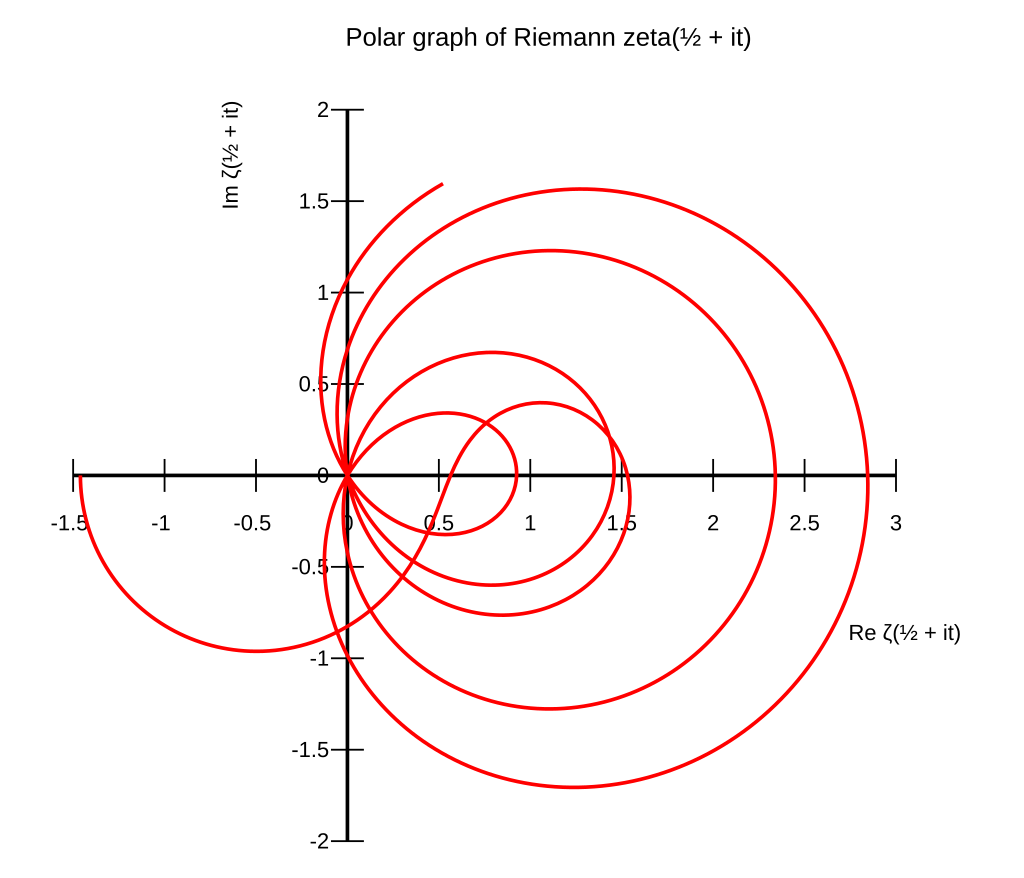
\includegraphics[width=0.6\textwidth]{figure/zeta.png}
%     \caption{Referensi Gambar}
%     \label{fig:3.ref_gbr}
%     {\footnotesize Sumber: internet}
% \end{figure}

% \subsection{Rumus} \label{II.mae}
% \textit{Mean Absolute Error} (MAE) \cite{Suryanto2019MAE} \cite{cort2005maermse}. Rumus perhitungan dari MAE dapat dilihat pada \ref{eq:2.mae}. \par

% \begin{equationcaptioned}[eq:2.mae]{
%     MAE = \frac{1}{n} \sum_{i=1}^{n} \left| y_i - \hat{y}_i \right|
% }{
%     Mean Absolute Error (MAE)
% }
% \end{equationcaptioned}